\documentclass[%
		%draft,
    %submission,
    %compressed,
    final,
    %
    %technote,
    %internal,
    %submitted,
    %inpress,
    reprint,
    %
    %titlepage,
    notitlepage,
    %anonymous,
    narroweqnarray,
    inline,
    twoside,
    invited
    ]{ieee}

\usepackage[utf8]{inputenc}
\usepackage[spanish]{babel}
\usepackage{graphicx}
\usepackage{verbatim}
\usepackage{moreverb}
\usepackage{amsmath}
\usepackage{amsfonts}
\usepackage{amssymb}
\usepackage{fancybox}
\usepackage{float}
\usepackage{fancyvrb}
\usepackage{subfigure}

\newcommand{\latexiie}{\LaTeX2{\Large$_\varepsilon$}}

%\usepackage{ieeetsp}    % if you want the "trans. sig. pro." style
%\usepackage{ieeetc}    % if you want the "trans. comp." style
%\usepackage{ieeeimtc}    % if you want the IMTC conference style

% Use the `endfloat' package to move figures and tables to the end
% of the paper. Useful for `submission' mode.
%\usepackage {endfloat}

% Use the `times' package to use Helvetica and Times-Roman fonts
% instead of the standard Computer Modern fonts. Useful for the 
% IEEE Computer Society transactions.
%\usepackage{times}
% (Note: If you have the commercial package `mathtime,' (from 
% y&y (http://www.yandy.com), it is much better, but the `times' 
% package works too). So, if you have it...
%\usepackage {mathtime}

% for any plug-in code... insert it here. For example, the CDC style...
%\usepackage{ieeecdc}

\begin{document}

%----------------------------------------------------------------------
% Title Information, Abstract and Keywords
%----------------------------------------------------------------------
\title[Redes Neuronales]{%
       Redes Neuronales}

% format author this way for journal articles.
% MAKE SURE THERE ARE NO SPACES BEFORE A \member OR \authorinfo
% COMMAND (this also means `don't break the line before these
% commands).
\author[Castiglione, Karpovsky, Sturla]{Gonzalo V. Castiglione, Alan E. Karpovsky, Martín Sturla\\\textit{Estudiantes 
       Instituto Tecnológico de Buenos Aires (ITBA)}\\
\textbf{19 de Abril de 2012}
}


\journal{Cátedra\ \ Sist.\ de\ Inteligencia\ Artificial,\ ITBA\ }
\titletext{-\ 19, ABRIL\ 2012}
\ieeecopyright{\copyright\ 2012 ITBA}
\lognumber{}
\pubitemident{}
\loginfo{19 de Abril, 2012.}
\firstpage{1}

\confplacedate{Buenos Aires, Argentina, 19 de Abril, 2012}

\maketitle               

\begin{abstract} 
El presente informe busca analizar  redes neuronales multicapa
con aprendizaje supervisado que resuelvan el problema del \textit{Simetría} y \textit{Paridad} lógica para $N$ bits 
con $2 \le N \le 5$ a través del uso de tres variantes de funciones de transferencia.

\end{abstract}

\begin{keywords}
perceptrón, función de transferencia, red neuronal, aprendizaje supervisado, conjunto de entrenamiento, conjunto de testeo
\end{keywords}

%----------------------------------------------------------------------
% SECTION I: Introduccion%----------------------------------------------------------------------
\section{Introducción}

\par Se analizó el comportamiento de distintas redes neuronales multicapa para el problema de la paridad y simetría booleana. 
Con este fin se implementó un algoritmo que permite definir la arquitectura y las propiedades de la red neuronal a generar de 
manera de hacer más simple y práctico su estudio. 

%----------------------------------------------------------------------
% SECTION II: Marco Teórico
%----------------------------------------------------------------------

\section{Desarrollo}

\subsection{Modelado del problema}

\par Se representó la red neuronal como una \textbf{matriz de pesos}. Cada neurona es una columna de pesos, cada capa de 
neuronas es una matriz de pesos, la red neuronal, por consiguiente, es un vector de matrices. Lo interesante es que hallar 
la salida de la red neuronal con una cierta entrada se reduce a multiplicar el vector entrada por cada una de estas matrices. Cabe destacar 
que al vector y a todos los pasos intermedios se les agrega siempre un $-1$ como último valor para el sesgo.\\

\par Para las unidades escalón el error está definido como la \textbf{Distancia Hamming Levenshtein}, para los 
otros tipos de unidades se decidió utilizar el \textbf{error cuadrático medio}.

\subsection{Features}

\par Se implementaron tres tipos de funciones para modificar la variable $\eta$ \textit{(learn rate)}: 
La primera de ellas es a valor \textbf{constante}, , la segunda es \textbf{\textit{annealed}} que reduce $\eta$ exponencialmente y por último se 
tiene un \textit{learning rate} \textbf{adaptative} que modifica $\eta$ en función de los últimos errores obtenidos. El crecimiento es aritmético, con cota 
en $\eta =0.5$, la reducción es exponencial.

\par Debido a la existencia de mínimos locales se desarrolló un algoritmo  \textbf{\textit{persistent search}} que dado un cierto error, entrena
 la red neuronal la cantidad de épocas especificada y verificar si el error obtenido es mayor al deseado. En cuyo caso 
reinicia el algoritmo, asigna los pesos al azar y vuelve a comenzar el entrenamiento.\\
\par Otra estrategia que se utilizó para subsanar este problema es la de darle un impulso a $\eta$ al detectar que el algoritmo está estancado 
en un mínimo local, haciendo que los valores de los pesos cambien significativamente en un paso (sería análogo a agregar poco ruido a todas la matrices).

\section{Resultados}

\par A modo de ejemplo, en la sección \textit{\textbf{Anexo A: Gráficos}} se muestran tres gráficos de los resultados obtenidos: En la \textit{Figura 1} 
se visualiza un estancamiento en un mínimo local debido al uso de unidades lineales, en la \textit{Figura 2} se puede apreciar 
cómo un $\eta$ dinámico puede, en algunos casos, ayudar a salir del mínimo local y por último en la \textit{Figura 3} se propone un ejemplo 
que ilustra cómo el $\eta$ varía a medida que el error decrece consitentemente.


\section{Conclusión}

\par En base a las pruebas podemos concluír que utilizando una función de transferencia \textit{lineal}, la red no aprenderá el problema. 
Esto se debe a que cada capa realiza una combinación lineal de la salida de la capa anterior, por lo que el resultado es combinación lineal de la entrada. 
Es decir que no existen coeficientes $a_1, a_2, \cdots, a_n$ que resuelvan, por ejemplo, la ecuación de paridad para $n$ bits, 
lo que hará que se tienda a un mínimo local o diverger en una secuencia alterna por lo que el error se incrementará indefinidamente, dependiendo del 
punto inicial y del valor de $\eta$.\\

\par A su vez, para las funciones escalón o no lineales se observó que es posible que ciertas arquitecturas tiendan a atascarse más en mínimos 
locales que otras. Para un XOR de $N$ bits, la arquitectura óptima resulta ser una única capa oculta con $N$ neuronas. 
Asimismo para el problema de simetría se sugiere utilizar una única capa oculta con 2 neuronas, 
independientemente de la cantidad de bits que contenga la entrada.


%\begin{thebibliography}{1}

%\bibitem{lamport1}
%Fierens, P. (2011),
%\newblock {\em Cuadrados mínimos: repaso},
%\newblock Buenos Aires: Instituto Tecnológico de Buenos Aires.

%\bibitem{lamport1}
%Abdi, H.,
%\newblock {\em  Least-squares: {Encyclopedia for research methods for the social sciences}},
%\newblock Thousand Oaks (CA): Sage. pp, 2003.

%\bibitem{lamport1}
%Farebrother, R.W. (1988),
%\newblock {\em Linear Least Squares Computations, STATISTICS: Textbooks and Monographs}, %\newblock New York: Marcel Dekker.

%\bibitem{lamport1}
%Lipson, M.; Lipschutz, S. (2001),
%\newblock {\em Schaum's outline of theory and problems of linear algebra}, 
%newblock New York: McGraw-Hill, pp. 69–80.


%\end{thebibliography}

%----------------------------------------------------------------------


\clearpage
\onecolumn

\section*{Anexo A: Gráficos}

\begin{figure}[H]
\begin{center}
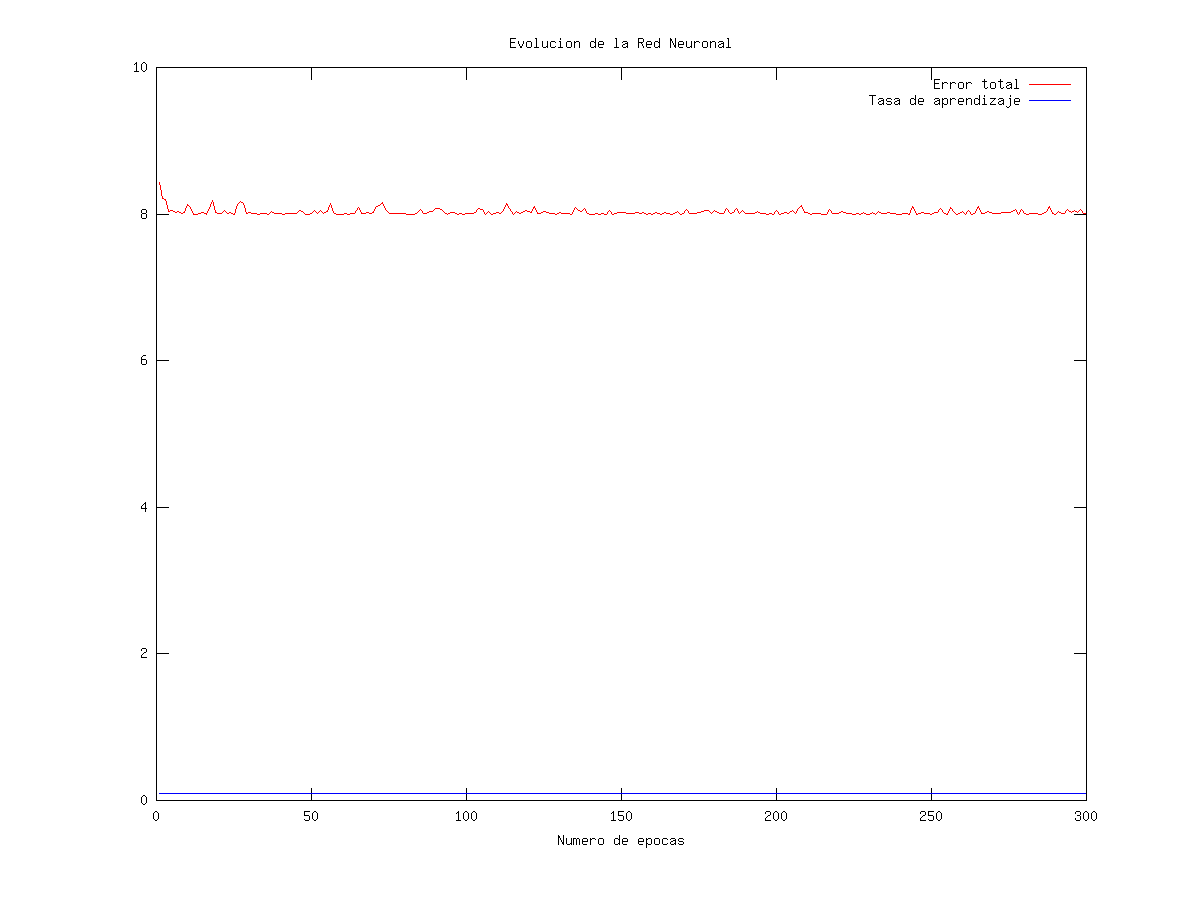
\includegraphics[scale=0.30]{./images/LinearConstante.png}
\label{modelado}
\end{center}
\end{figure}

\begin{center}
\par Figura 1: Ejemplo de estancamiento en mínimo local debido a la utilización de una función de transferencia lineal.
\end{center}

\begin{figure}[H]
\begin{center}
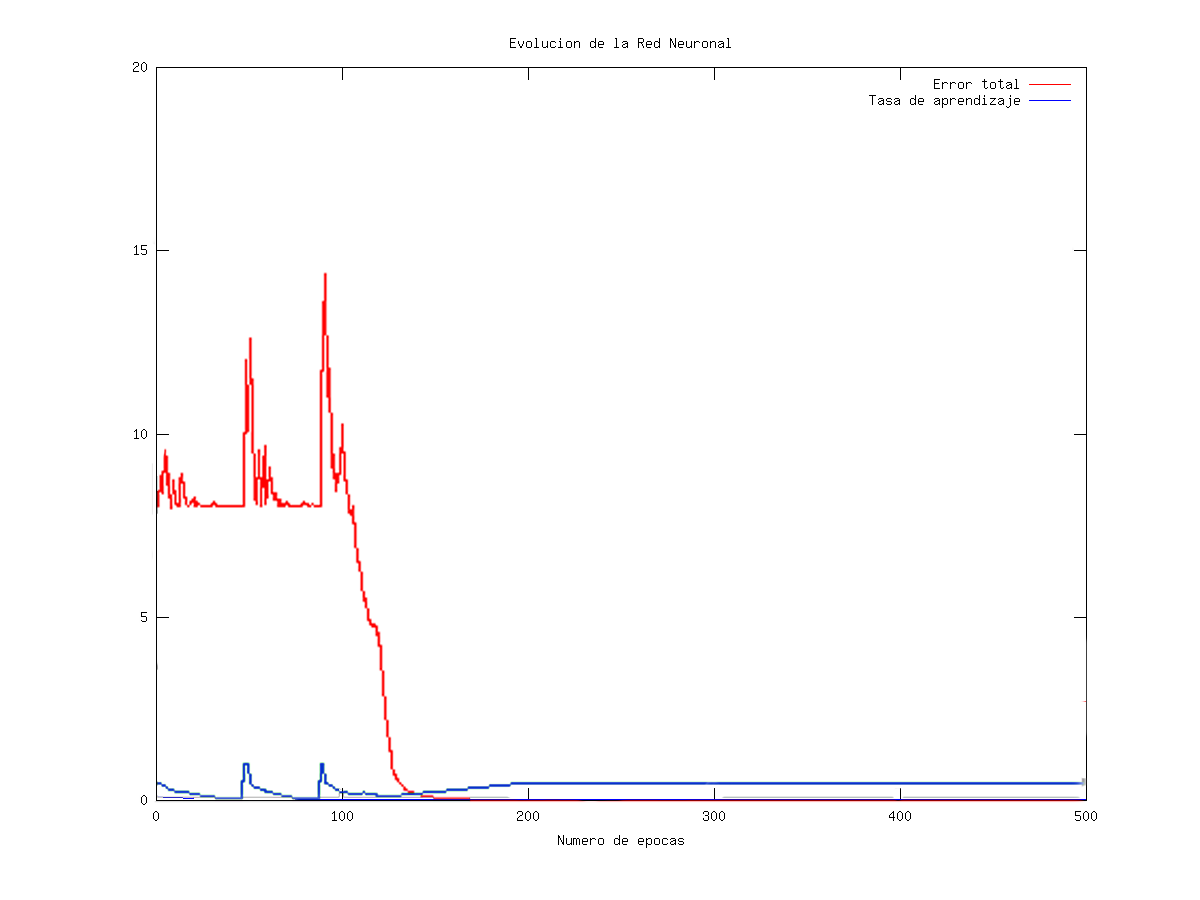
\includegraphics[scale=0.30]{./images/escapeminlocal.png}
\label{modelado}
\end{center}
\end{figure}

\begin{center}
\par Figura 2: Escape de mínimo local utilizando eta dinámico para el problema de paridad de 3 bits usando 500 épocas y una arquitectura de una capa oculta con 3 neuronas.
\end{center}

\clearpage

\begin{figure}[H]
\begin{center}
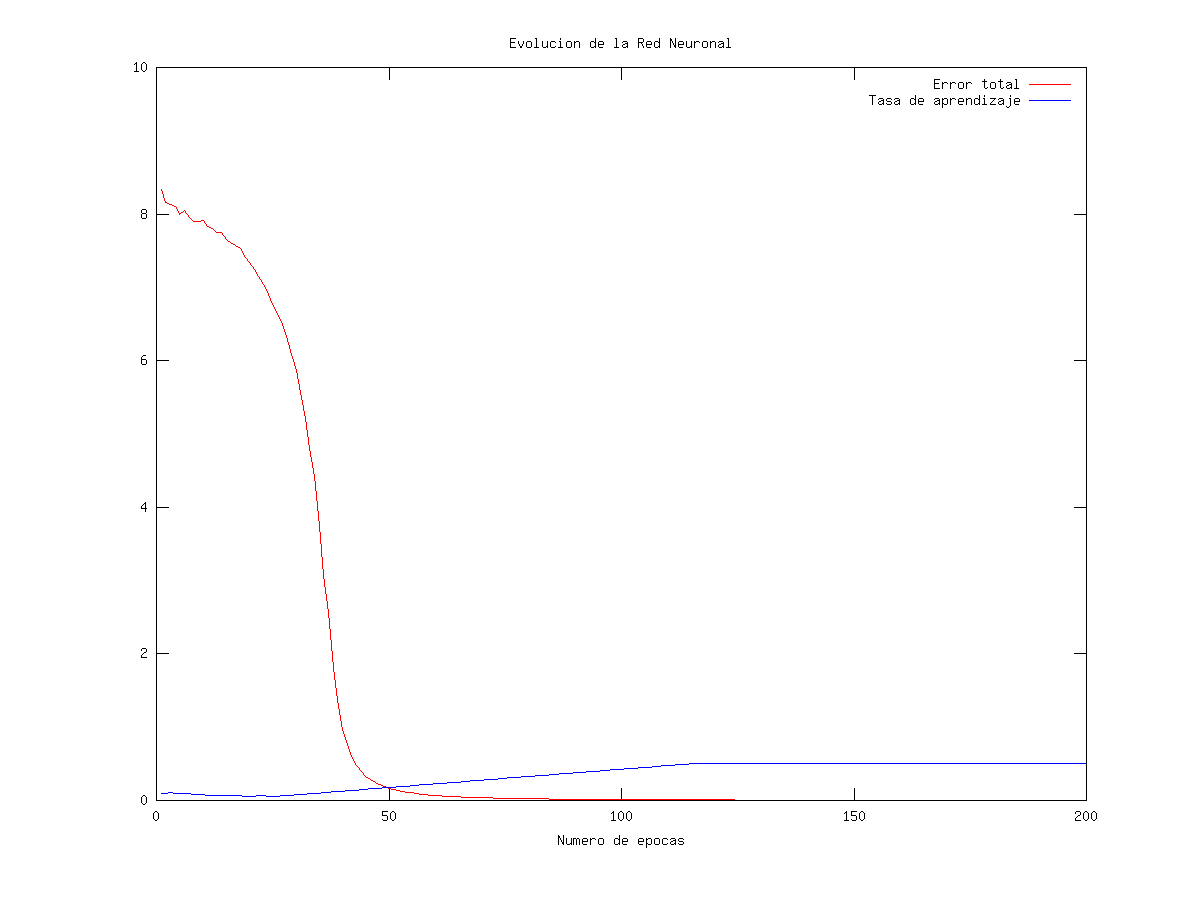
\includegraphics[scale=0.30]{./images/incremento.png}
\label{modelado}
\end{center}
\end{figure}

\begin{center}
\par Figura 3: Muestra cómo se incrementa hasta el valor máximo eta cuando la red neuronal resuelve el problema con el error deseado.
\end{center}




%\VerbatimInput{./code/calculoAb.m}




\end{document}